\chapter{Object detection}


\begin{description}
    \item[Object detection] \marginnote{Object detection}
        Given an RGB $W \times H$ image, determine a set of objects $\{ o_1, \dots, o_n \}$ contained in it. Each object $o_j$ is described by:
        \begin{itemize}
            \item A category $c_j \in \{ 1, \dots, C \}$ as in image classification.
            \item A bounding box $BB_j = [ x_j, y_j, w_j, h_j ]$ where $x_j, w_j \in [0, W-1]$ and $y_j, h_j \in [0, H-1]$. ($x_j$, $y_j$) is the center and ($w_j$, $h_j$) is the size of the box.
            \item A confidence score $\rho_j$.
        \end{itemize}

        \begin{figure}[H]
            \centering
            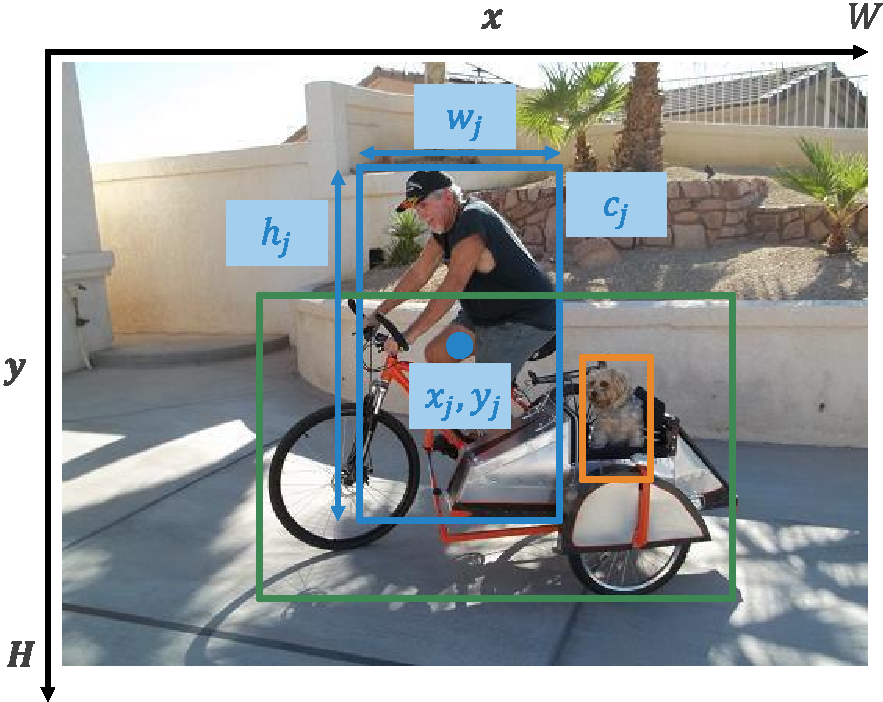
\includegraphics[width=0.45\linewidth]{./img/_object_detection_example.pdf}
        \end{figure}

        \begin{remark}
            Differently from classification, a model has to:
            \begin{itemize}
                \item Be able to output a variable number of results.
                \item Output both categorical and spatial information.
                \item Work on high resolution input images.
            \end{itemize}
        \end{remark}
\end{description}



\section{Metrics}

\begin{description}
    \item[Intersection over union (\texttt{IoU})] 
    \marginnote{Intersection over union (\texttt{IoU})}
        Measures the amount of overlap between two boxes computed as the ratio of the area of intersection over the area of union:
        \[ \texttt{IoU}(BB_i, BB_j) = \frac{\vert BB_i \cap BB_j \vert}{\vert BB_i \vert + \vert BB_j \vert - \vert BB_i \cup BB_j \vert} \]

        \begin{description}
            \item[True/false positive criteria] 
                Given a threshold $\rho_\texttt{IoU}$, a detection $BB_i$ is a true positive (\texttt{TP}) w.r.t. a ground truth $\hat{BB_j}$ if it is classified with the same class and:
                \[ \texttt{IoU}(BB_i, \hat{BB_j}) > \rho_\texttt{IoU} \]

                \begin{remark}
                    Confidence can also be considered when determining a match through a threshold $\rho_\text{min}$.
                \end{remark}
        \end{description}

    \item[Recall]
        Measures the number of ground truth objects that have been found:
        \[ \texttt{recall} = \frac{\vert \texttt{TP} \vert}{\vert \text{ground truth boxes} \vert} \]

    \item[Precision]
        Measures the number of correct detections among all the predictions:
        \[ \texttt{precision} = \frac{\vert \texttt{TP} \vert}{\vert \text{model detections} \vert} \]

    \begin{figure}[H]
        \centering
        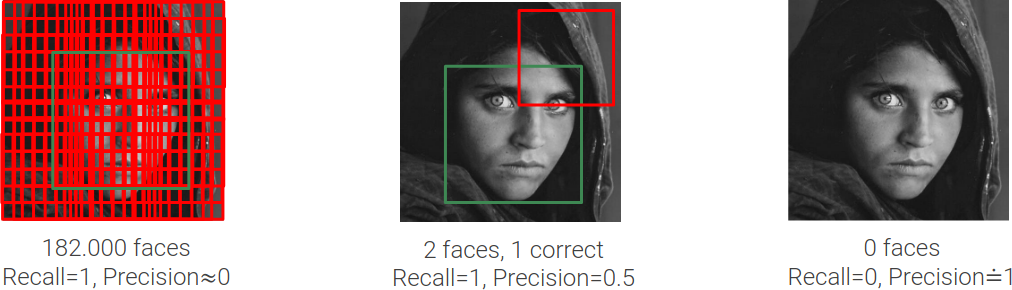
\includegraphics[width=0.7\linewidth]{./img/obj_det_recall_precision.png}
        \caption{
            Recall and precision in different scenarios
        }
    \end{figure}

    \item[Precision-recall curve]
        Plot that relates precision and recall.

        \begin{example}
            Consider the following image and the bounding boxes found by a detector:
            \begin{figure}[H]
                \centering
                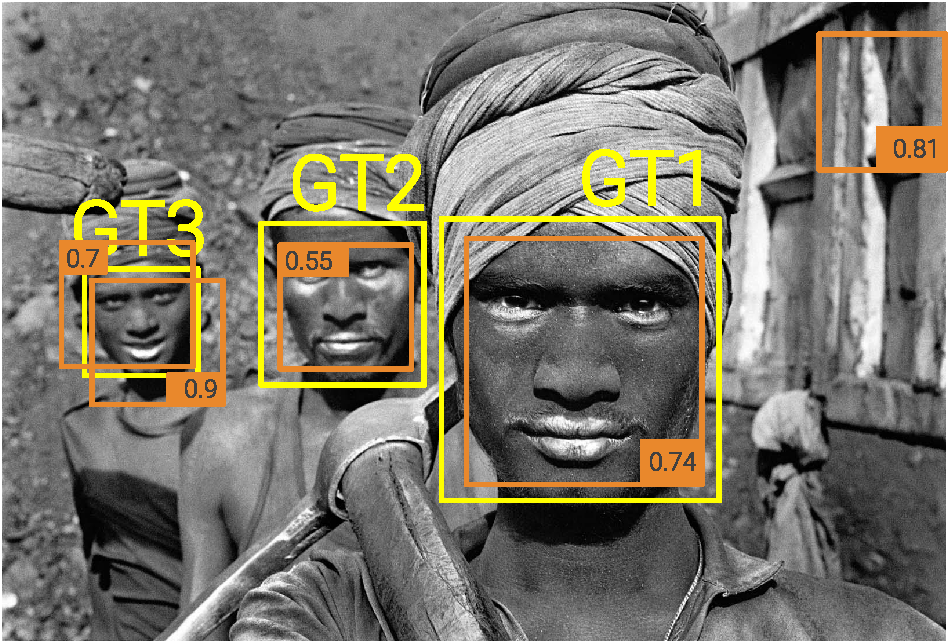
\includegraphics[width=0.4\linewidth]{./img/_example_precision_recall_curve1.pdf}
                \caption{
                    \parbox[t]{0.6\linewidth}{
                        Ground truth (yellow boxes) and predictions (orange boxes) with their confidence score
                    }
                }
            \end{figure}

            By sorting the confidence scores, it is possible to plot the precision-recall curve by varying the threshold $\rho_\text{min}$:
            \begin{figure}[H]
                \centering
                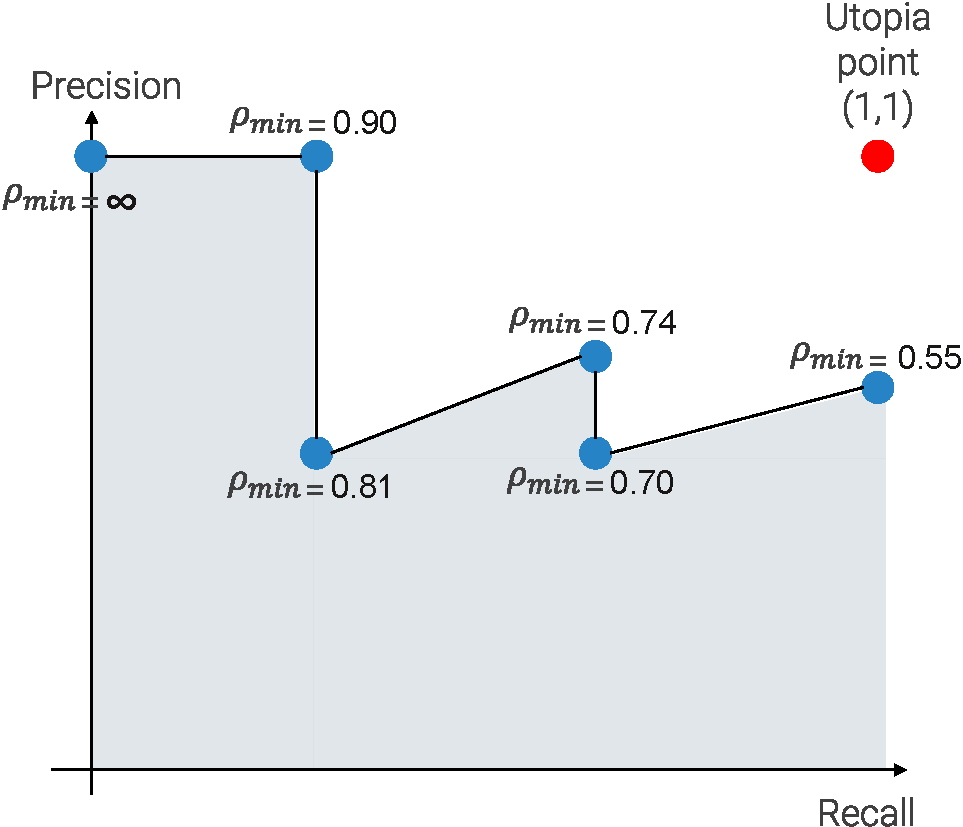
\includegraphics[width=0.4\linewidth]{./img/_example_precision_recall_curve2.pdf}
            \end{figure}

            \indenttbox
            \begin{remark}
                Recall is monotonically decreasing, while precision can both decrease and increase.
            \end{remark}
        \end{example}
\end{description}